

\tikzset{every picture/.style={line width=0.75pt}} %set default line width to 0.75pt        

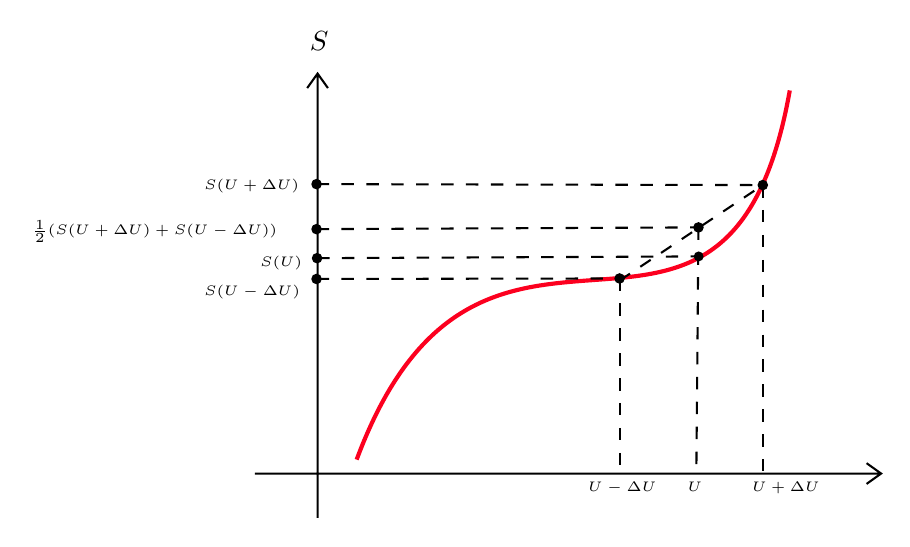
\begin{tikzpicture}[x=0.75pt,y=0.75pt,yscale=-1,xscale=1]
%uncomment if require: \path (0,300); %set diagram left start at 0, and has height of 300

%Shape: Axis 2D [id:dp8371481886954371] 
\draw  (151,247.72) -- (452.68,247.72)(181.17,55) -- (181.17,269.13) (445.68,242.72) -- (452.68,247.72) -- (445.68,252.72) (176.17,62) -- (181.17,55) -- (186.17,62)  ;
%Curve Lines [id:da9915347598713424] 
\draw [color={rgb, 255:red, 252; green, 0; blue, 31 }  ,draw opacity=1 ][line width=1.5]    (200,241) .. controls (260.68,78.13) and (378.68,232.13) .. (408.68,63.13) ;
%Straight Lines [id:da5338080977523495] 
\draw  [dash pattern={on 4.5pt off 4.5pt}]  (326.68,153.73) -- (326.68,247.43) ;
\draw [shift={(326.68,153.73)}, rotate = 90] [color={rgb, 255:red, 0; green, 0; blue, 0 }  ][fill={rgb, 255:red, 0; green, 0; blue, 0 }  ][line width=0.75]      (0, 0) circle [x radius= 2.01, y radius= 2.01]   ;
%Straight Lines [id:da5315894348525821] 
\draw  [dash pattern={on 4.5pt off 4.5pt}]  (364.68,129.13) -- (363.68,245.95) ;
\draw [shift={(364.68,129.13)}, rotate = 90.49] [color={rgb, 255:red, 0; green, 0; blue, 0 }  ][fill={rgb, 255:red, 0; green, 0; blue, 0 }  ][line width=0.75]      (0, 0) circle [x radius= 2.01, y radius= 2.01]   ;
%Straight Lines [id:da8144040544764883] 
\draw  [dash pattern={on 4.5pt off 4.5pt}]  (395.68,108.73) -- (395.68,247.57) ;
\draw [shift={(395.68,108.73)}, rotate = 90] [color={rgb, 255:red, 0; green, 0; blue, 0 }  ][fill={rgb, 255:red, 0; green, 0; blue, 0 }  ][line width=0.75]      (0, 0) circle [x radius= 2.01, y radius= 2.01]   ;
%Straight Lines [id:da6789218420069354] 
\draw  [dash pattern={on 4.5pt off 4.5pt}]  (326.68,154.73) -- (395.68,108.73) ;
%Shape: Circle [id:dp49363498746891266] 
\draw  [fill={rgb, 255:red, 0; green, 0; blue, 0 }  ,fill opacity=1 ] (362.93,143.11) .. controls (362.93,142.09) and (363.76,141.26) .. (364.78,141.26) .. controls (365.8,141.26) and (366.63,142.09) .. (366.63,143.11) .. controls (366.63,144.14) and (365.8,144.97) .. (364.78,144.97) .. controls (363.76,144.97) and (362.93,144.14) .. (362.93,143.11) -- cycle ;
%Straight Lines [id:da07316386568730371] 
\draw  [dash pattern={on 4.5pt off 4.5pt}]  (180.68,153.97) -- (326.68,153.73) ;
\draw [shift={(180.68,153.97)}, rotate = 359.91] [color={rgb, 255:red, 0; green, 0; blue, 0 }  ][fill={rgb, 255:red, 0; green, 0; blue, 0 }  ][line width=0.75]      (0, 0) circle [x radius= 2.01, y radius= 2.01]   ;
%Straight Lines [id:da8730317034140778] 
\draw  [dash pattern={on 4.5pt off 4.5pt}]  (180.68,129.97) -- (363.68,129.13) ;
\draw [shift={(180.68,129.97)}, rotate = 359.74] [color={rgb, 255:red, 0; green, 0; blue, 0 }  ][fill={rgb, 255:red, 0; green, 0; blue, 0 }  ][line width=0.75]      (0, 0) circle [x radius= 2.01, y radius= 2.01]   ;
%Straight Lines [id:da3224382986728025] 
\draw  [dash pattern={on 4.5pt off 4.5pt}]  (180.68,108.28) -- (395.68,108.73) ;
\draw [shift={(180.68,108.28)}, rotate = 0.12] [color={rgb, 255:red, 0; green, 0; blue, 0 }  ][fill={rgb, 255:red, 0; green, 0; blue, 0 }  ][line width=0.75]      (0, 0) circle [x radius= 2.01, y radius= 2.01]   ;
%Straight Lines [id:da003959848940690458] 
\draw  [dash pattern={on 4.5pt off 4.5pt}]  (180.93,143.95) -- (363.93,143.11) ;
\draw [shift={(180.93,143.95)}, rotate = 359.74] [color={rgb, 255:red, 0; green, 0; blue, 0 }  ][fill={rgb, 255:red, 0; green, 0; blue, 0 }  ][line width=0.75]      (0, 0) circle [x radius= 2.01, y radius= 2.01]   ;

% Text Node
\draw (176,33.4) node [anchor=north west][inner sep=0.75pt]    {$S$};
% Text Node
\draw (358,250.4) node [anchor=north west][inner sep=0.75pt]  [font=\tiny]  {$U$};
% Text Node
\draw (389,250.4) node [anchor=north west][inner sep=0.75pt]  [font=\tiny]  {$U+\Delta U$};
% Text Node
\draw (310,250.4) node [anchor=north west][inner sep=0.75pt]  [font=\tiny]  {$U-\Delta U$};
% Text Node
\draw (125,104.4) node [anchor=north west][inner sep=0.75pt]  [font=\tiny]  {$S(U+\Delta U)$};
% Text Node
\draw (125,155.4) node [anchor=north west][inner sep=0.75pt]  [font=\tiny]  {$S(U-\Delta U)$};
% Text Node
\draw (42,124.4) node [anchor=north west][inner sep=0.75pt]  [font=\tiny]  {$\frac{1}{2}\qty( S( U+\Delta U) +S( U-\Delta U))$};
% Text Node
\draw (152,141.4) node [anchor=north west][inner sep=0.75pt]  [font=\tiny]  {$S(U)$};


\end{tikzpicture}
